\chapter{XML Indexing}
Elaborare una query XPath significa visitare il documento e restituire i nodi che rispondo alle proprietà desiderate; nella visualizzazione ad albero del DOM questo corrisponde a una visita in profondità. Per documenti molto grandi tuttavia questa visita diventa molto onerosa anche per query molto semplici. Lo scopo degli indici XML è quello di semplificare l'operazione riducendo lo spazio e il tempo di ricerca in qualche modo.\\
Da un punto di vista formale Xpath è un linguaggio con una certa espressività in grado di distinguere tutti gli elementi di un documento ma una query molto spesso non utilizza a pieno tutto il potere espressivo a disposizione. Avremo allora delle classi di query per le quali alcuni nodi saranno indistinguibili. Un indice non è altro che una struttura dati in cui i nodi non distinguibili vengono accorpati, fornendo così una struttura dati semplificata su cui valutare le query. Va notato che a volte può essere utile utilizzare un indice anche se la risposta alla query risulterà non accurata (avremo dei "falsi positivi") per poi effettuare un filtraggio dei risultati.\\\\
In questa sezione vedremo alcuni tipi di indici strutturali per documenti XML basati sui nodi e sui grafi.
\section{Indici Basati sui Nodi}
Inteval e Path Labeling sono techiche di indicizzazione basate sui nodi. Immagazzinando dei valori che riflettono in qualche modo la posizione dei nodi nella struttura dell'albero XML di trovare, dato un nodo, il nodo padre, i figli, i fratelli, i discendenti e gli antenati. Mostriamo due varianti dette \emph{Interval(o Region) Labeling} e \emph{il Prefix(o Path) Labeling} che differiscono nel etichettamento.

\subsection{Interval Labeling}
Inteval Labeling significa etichettare i nodi con un intervallo in base alla posizione nell'albero o nel documento. Esempi di questo metodo sono la tecnica \emph{(Pre,Post)} e la tecnica \emph{(Beg,End)} che vedremo in dettaglio.
\\
Nel metodo \emph{(Pre,Post)} visitiamo l'albero XML con un algoritmo di visita Pre-Order e Post-Order. Ogni volta che incontriamo un nodo lo numeriamo con la posizione di visita. Confrontando le etichette possiamo ricostruire la posizione di ogni nodo nell'albero senza mantenere la struttura dati in memoria.
\\
Nel metodo \emph{(Beg,End)} scorriamo il documento XML in maniera sequenziale mantenendo un contatore che viene incrementato ogni qual volta incontriamo un tag, un attributo, o i valori a essi associati. Assegniamo il valore del contatore all'etichetta \emph{Beg} dell'elemento quando lo incontriamo e quando giungiamo alla terminazione di questo assegniamo il valore del contatore a \emph{End}.
\\\\
\begin{example}
\begin{figure}[h]
\centering
\subfloat[]{
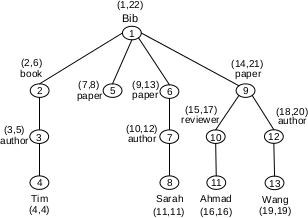
\includegraphics[scale=.7]{begend1}
}
\subfloat[]{
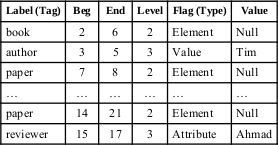
\includegraphics[scale=.7]{begend2}
}
\caption{esempio di labeling (beg,end)}
\end{figure}
\end{example}
\\
Aggiungendo una terza etichetta \emph{Level} che indica la profondità nell'albero possiamo formulare due regole per calcolare le relazioni successore-discendente e padre-figlio:
\begin{itemize}
\item \textbf{Proprietà 1:} in un albero un nodo $x$ è antenato di un nodo $y$ sse $x.Beg < y.Beg < x.End$
\item \textbf{Proprietà 2:} in un albero un nodo $x$ è padre di un nodo $y$ sse $x.Beg < y.Beg < x.End$ and $y.Level = x.Level + 1$
\end{itemize}

\subsection{Path Labeling}
Questa tecnica si basa sull'etichettare ogni nodo con un vettore in cui è indicato il percorso fino ad esso. Come esempio di questa tecnica illustreremo il metodo Dewey.
\\
Il metodo Dewey prevede che ogni etichetta rappresenti la posizione del nodo includendo come prefisso la codifica dei suoi antenati (coordinata verticale) e aggiungendo il numero del nodo tra i suoi fratelli (coordinata orizzontale). Il livello è implicitamente definito dalla lunghezza del vettore.
Per stabilire le relazioni tra due nodi sarà sufficiente effettuare un controllo di pattern matching tra le etichette.
\\
Gli antenati di un certo nodo x saranno tutti quelli la cui etichetta è una sotto-stringa dell'etichetta di x, il padre sarà il nodo la cui etichetta è soltanto un carattere più breve; ad esempio è facile verificare che il nodo $(0.3)$ è antenato del nodo $(0.3.1.0)$ e padre di $(0.3.1)$.
\\
I fratelli invece avranno un etichetta della stessa lunghezza che differirà soltanto per l'ultimo carattere; ad esempio $(0.3.1)$ e $(0.3.2)$.
\\
Il punto di forza di questo sistema è la semplicità nella verifica delle relazione e nell'aggiornamento della struttura; la grande debolezza invece la lunghezza delle etichette cresce con l'aumentare delle profondità e con essa lo spazio necessario ad immagazzinare le informazioni e il tempo necessario a calcolare le relazioni tra i nodi.
\section{Strong DataGuide}
Proposto nel 1997 da Goldman e Widom, è uno dei primi algoritmi utilizzati per il calcolo degli indici. Partendo da un grafo $G_1$, Strong DataGuide restituisce un grafo $G_2$ in cui i nodi vengono partizionati in base al percorso dalla radice al nodo. Pensando il grafo di partenza come un automa a stati finiti \textbf{non-deterministico} l'algoritmo genera il grafo dell'automa a stati finiti \textbf{deterministico} corrispondente.\\
Un indice Strong DataGuide deve soddisfare le seguenti caratteristiche di base:
\begin{itemize}
\item Ogni cammino distinto radice-nodo nel grafo di partenza compare soltanto una volta nell'indice.
\item Ogni singolo cammino nel grafo indice deve avere almeno una corrispondenza nel grafo originale, ossia non ci sono percorsi non validi nell'indice.
\end{itemize}
Essere deterministico è contemporaneamente un vantaggio e uno svantaggio in quanto i nodi con più di un padre(idref) verranno duplicati. Se consideriamo un documento con idref modellato quindi come un DAG esiste la possibilità che la cardinalità dell'indice sia maggiore di quella del grafo di partenza, vanificando lo scopo dello stesso. Nel caso invece di un documento modellato come un albero nel caso peggiore la cardinalità dell'indice sarà uguale a quella del documento.\\\\
DataGuide è in grado di fornire risposte precise e complete alle cosìdette path-query, cioè quelle query che presentano sono relazioni padre-figlio o antenato-discendente. Nel caso di query che coinvolgono anche i predicati (twig-query) la risposta ottenuta sarà completa ma non precisa e otterremo dei falsi positivi.\\\\
\begin{example}
\begin{figure}[H]
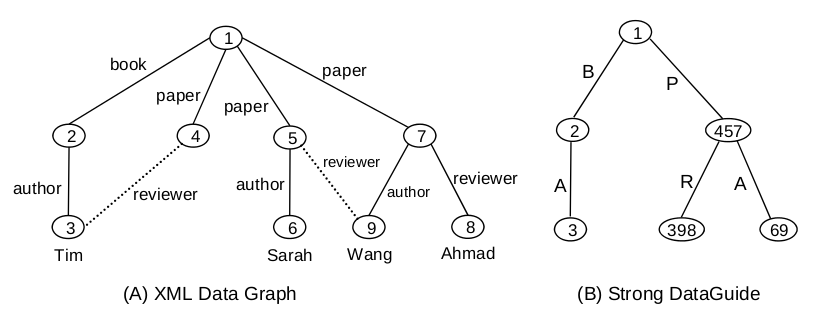
\includegraphics[scale=.5]{dataguide}
\end{figure}
\end{example}
\section{Indici Basati sulla Bisimulazione}
\section{Indici Basati sulla Simulazione}